\documentclass[herrin-thesis.tex]{subfiles}
\begin{document}

\section{Motivation}
\label{sec:muon:motivation}
One potential source of background in EXO-200 is unstable isotopes of common elements, created by neutron activation. The largest source of these neutrons is spallation by cosmic ray muons. Indeed, EXO-200 is located underground to reduce cosmic activation. The energy loss rate \((d E/d x)\) for relativistic muons has a broad minimum between \SIlist{1;10}{\GeV}, and increases slowly for higher energies. Therefore, some muons produced in the upper atmosphere can still travel deep underground.

Neutrons from these muons can capture on detector materials or the HFE, producing high-energy gamma rays that might Compton scatter in the detector and leave behind energy close to the Q value for \xenon{136}. These gamma rays are prompt, and so can be vetoed if the muon can be tagged. A neutron capture on \xenon{136} produces \xenon{137}, an isotope that beta decays with a Q value of 3.8 MeV, which means the beta particle produced in the decay could have an energy close to the Q value of \xenon{136}. The half life of \xenon{136} is 3.8 minutes, and so vetoing becomes more difficult. But a good measurement of the muon flux can put constraints on the amount of \xenon{137} decays observed.

\section{Identifying Muons}
\label{sec:muon:id}
Muons that reach underground have typical energies of \SIrange{1}{100}{\GeV}, a range in which they are minimally ionizing. Those that pass through the detector typically leave a straight line of ionization along their path. Like any energy deposition in EXO-200, some of the energy deposited becomes scintillation light, while the remaining ionization is drifted and collected. Thus, a muon passing through EXO-200 will show a bright flash of light, followed by ionization across many wire channels, linearly spread in time. \Cref{fig:muon:eventdisplay} shows a typical example. This distinct linear trail provides a means to tag the muon.

\begin{figure}[htbp]
\centering
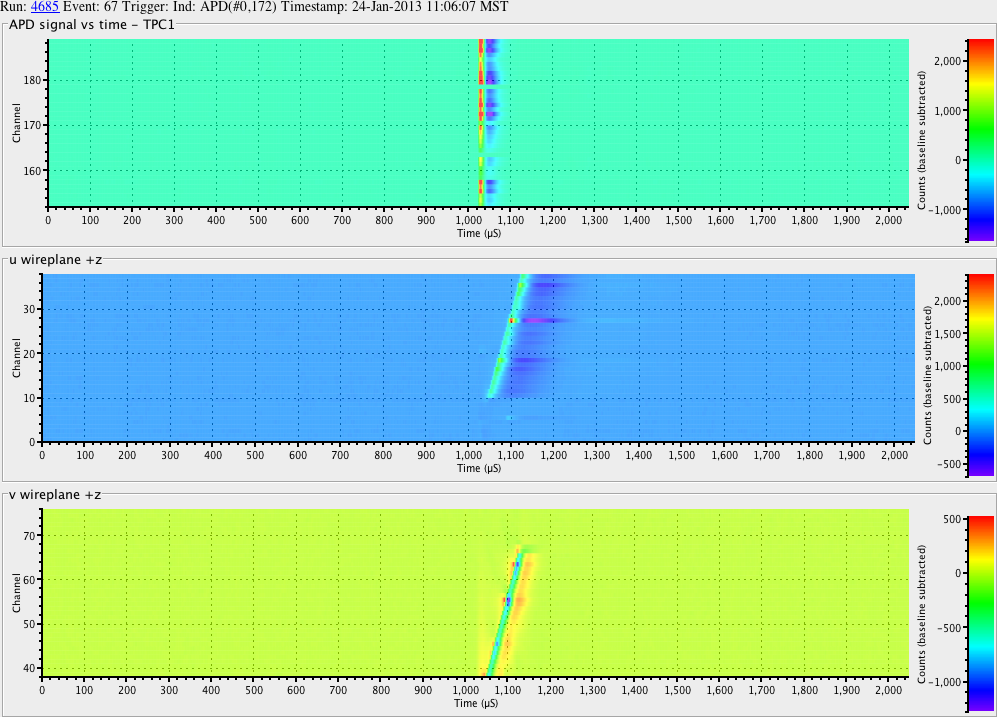
\includegraphics[width=1\columnwidth]{./plots/muon_eventdisplay_run_4685_ev_67.png}
\caption[A muon passing through EXO-200]{The event display for a muon passing through EXO-200. The upper panel shows the APDs versus time, displaying the flash of light when the muon passes through. The middle (lower) panel shows u (v) wire channels versus time, showing the characteristic linear trail of ionization.}
\label{fig:muon:eventdisplay}
\end{figure}

\subsection{Identifying Muons with the Hough Transform}
The Hough transform\cite{Hough:1959fk}\cite{Duda:1972:UHT:361237.361242} is an algorithm originally used to look for tracks in bubble chamber photos. A line can be completely parameterized by the angle \(\eta\) it makes with an axis, and the perpendicular distance \(r\) from the line to the origin. The Hough transform maps a pixel in an image to all possible lines that can pass through that pixel, which looks like a sinusoidal curve in \((\eta, r)\) space. If some of the pixels form a line, then these curves will converge at the point corresponding to that line.

This can be applied to EXO-200 to look for muons. First, ionization deposits are identified by simply looking at the collection wire channel waveforms and looking for the waveform rising a set threshold above its baseline. A ``hot spot'' is associated with the time value at which the waveform peaks above this threshold. The induction wires are analyzed the same way, except looking for the waveform dipping below its baseline. The Hough-transformed hot spots are placed in a histogram, and the bin with the most entries is used to reconstruct the projection of the muon's track onto the wire planes. \Cref{fig:muon:houghtransform} shows an example.

\begin{figure}[htbp]
\centering
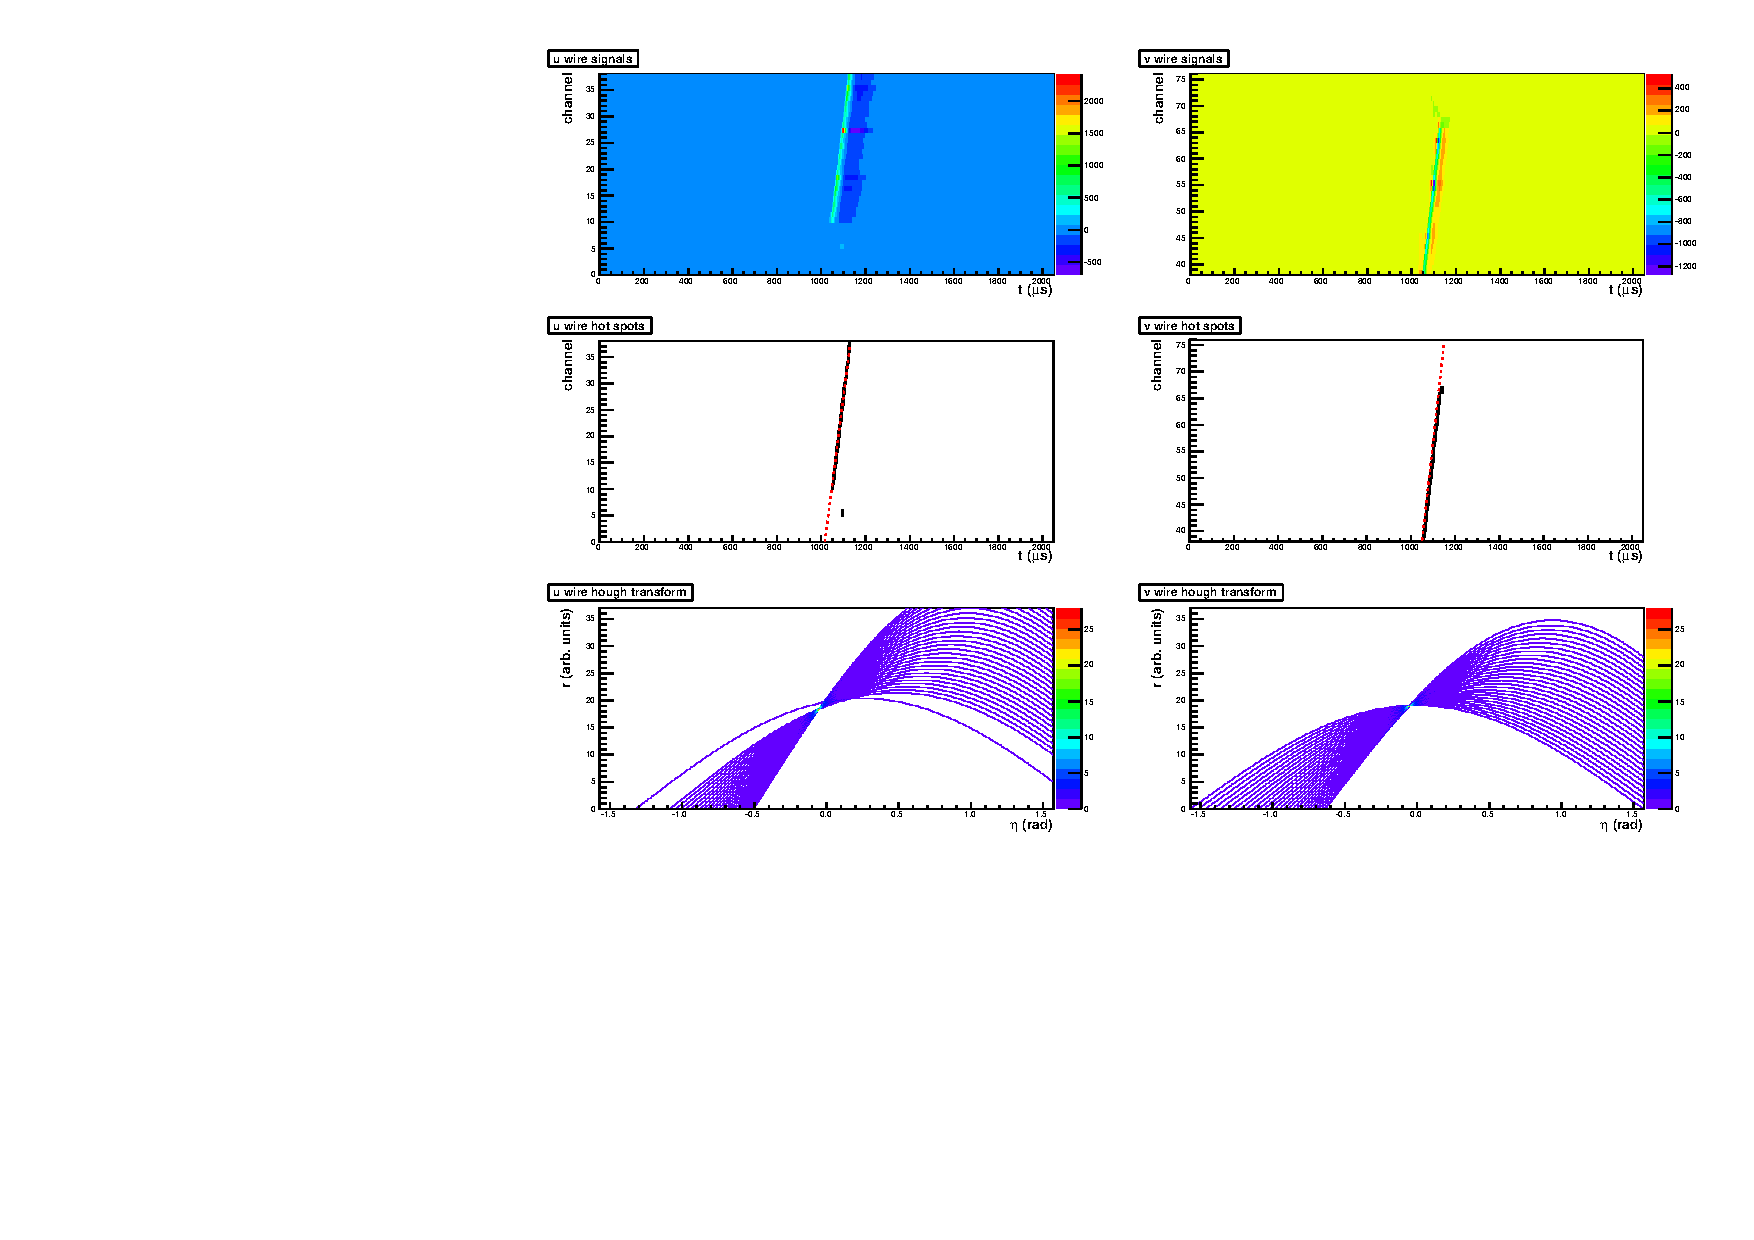
\includegraphics[width=1\columnwidth]{./plots/muon_houghtransform_run_4685_ev_67.pdf}
\caption[Identifying a muon with the Hough transform]{The Hough transform used to identify and reconstruct a muon passing through EXO-200. The left side shows collection wire channels, and the right side shows induction wire channels. The upper panels show the raw waveforms, baseline subtracted. The middle panels shows the identified hot spots in the waveforms in black, and the reconstructed tracks in red. The lower panels show the Hough transforms of the hot spots above, which converge on the point corresponding to the red line above.}
\label{fig:muon:houghtransform}
\end{figure}

After passing a check for noise (described in \Cref{app:noisetagger}) and a check for a large amount of scintillation light, an event will be tagged as a muon if it has good tracks in both the induction and collection wire planes in at least one TPC. A ``good'' track must be reconstructed from at least 5 hot spots that lie along the reconstructed track, or at least 3 hot spots along the track if fewer than 5 total spots were found.

The Hough transform reconstructs the projection of the muon's path onto the wire planes. Since the drift velocity and wire spacings are well known, these projections can be translated back to an incident angle for the muon.

\subsection{Validation with Monte Carlo Simulations}
In order to validate this muon tagging algorithm, 2 million muons were generated in the EXOSim GEANT4 simulation of the EXO-200 detector. The overall efficiency of the tagging depends on the angular distribution of the incident muons (for example, one could imagine a pathological scenario in which all muons were parallel to the wires in one plane). The angular distribution underground is approximated\cite{miyake:1973} by
\begin{equation}
\label{eq:muon_angular_distribution}
\frac{dN}{d\Omega} \propto \left (\cos \theta \right)^{1.53}e^{-8\times10^{-4} h \left(\sec \theta -1\right)}
\end{equation}
where \(\theta\) is the zenith angle and \(h\) is the vertical depth in \si{\hecto\gram\per\square\centi\meter} (\SI{1}{\hecto\gram\per\square\centi\meter} is equivalent shielding to one meter of water). For WIPP, previous experiments have measured \(h\) to be \(1585^{+11}_{-6}\) \si{\hecto\gram\per\square\centi\meter}\cite{Esch:2004zj}. This distribution is a good approximation for \(\theta < \pi/3\).

The energy distribution for muons underground can also be approximated\cite{Gaisser:1990kx}. The distribution for muons at the surface is given by
\begin{equation}
\label{eq:muon_surface_distribution}
\frac{dN}{dE} \propto E^{-2.7}\left(\frac{1}{1+\frac{1.1 E \cos \theta}{115}} + \frac{0.054}{1+\frac{1.1 E \cos \theta}{850}}\right)
\end{equation}
for \(E\) in \si{\GeV}. The flux underground is then
\begin{equation}
\label{eq:muon_underground_distribution}
\frac{dN}{dE} = \frac{dN}{dE_0}e^{b h \sec \theta}
\end{equation}
where \(b E\) defines the rate of continuous energy loss for muons. \(b\) is about \SI{4d-6}{\g\per\square\cm} for standard rock. This makes the substitution
\begin{equation}
\label{eq:muon_E0_def}
E_0 = e^{b h \sec \theta}\left(E + \epsilon\right) - \epsilon
\end{equation}
which is the average energy of surface muons that pass through \(h\sec\theta\) of material and emerge with energy \(E\). The parameter \(\epsilon\) is a critical energy above which discrete energy losses dominate, rather than continuous losses described by \(b\). For standard rock, \(\epsilon\) is about \SI{693}{\GeV}\cite{groom:2001ys}.

Muon events were simulated by first picking an azimuthal angle \(\phi\) uniformly from \(\left(-\pi, \pi\right]\) and a zenith angle \(\theta\) from \cref{eq:muon_angular_distribution}. The energy was selected in a range of \SIrange{1}{1000}{\GeV} from \cref{eq:muon_underground_distribution} for the selected zenith angle. A point was chosen uniform randomly in the cylindrical TPC volume, and a muon was generated \SI{3}{\meter} from this point with the selected energy and incident angles. Positively charged muons were generated in a 1.25 ratio to negatively charged muons. The ``standard rock'' values for \(b\) and \(\epsilon\) were used, and the depth \(h\) was varied 5\% around \SI{1585}{\hecto\gram\per\square\centi\meter} to account for systematic effects of the angular distribution on efficiency.

\subsection{Reconstruction Accuracy}
For most incident muon angles, the algorithm correctly reconstructs their incident angle. \Cref{fig:muon_misrecon_rate} shows the rate for muons to be misreconstructed more than \ang{5} from their true angle. This analysis concentrates on the region with good angular reconstruction. This region is bounded by the polygon with vertices \((\theta, \phi) = \{(0.4, 0), (0.45, 0.15), (0.45, 0.9), (0.75, 1.2), (0.95, 1.2), (1.3, 0.1)\}\) and their reflection  across \(\phi=0\), as well as the symmetric region on the opposite side of the detector.
 \begin{figure}[htpb]
 \centering
 \begin{subfigure}[b]{1.0\textwidth}
 \centering
 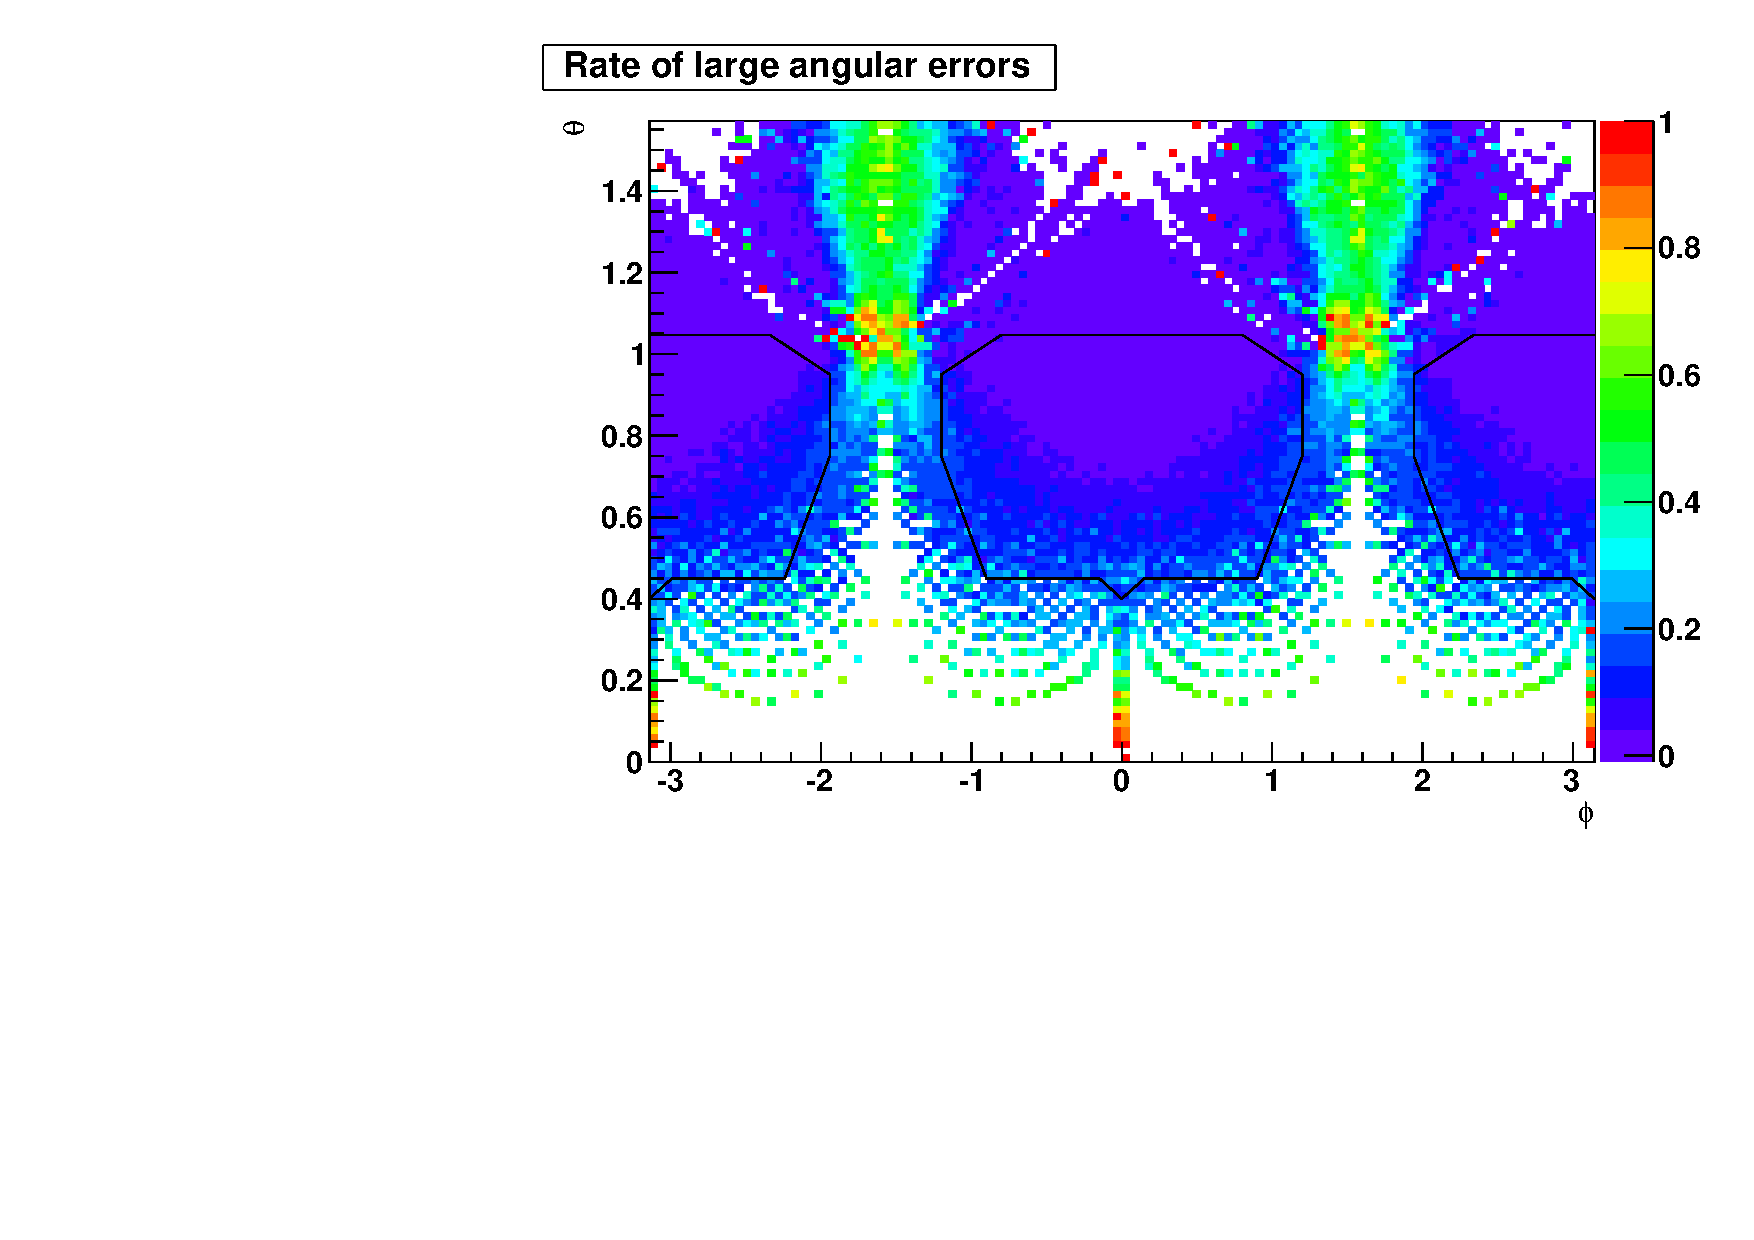
\includegraphics[width=0.8\textwidth]{./plots/muon_misrecon_ang_rate.pdf}
 \end{subfigure}
  \begin{subfigure}[b]{1.0\textwidth}
  \centering
   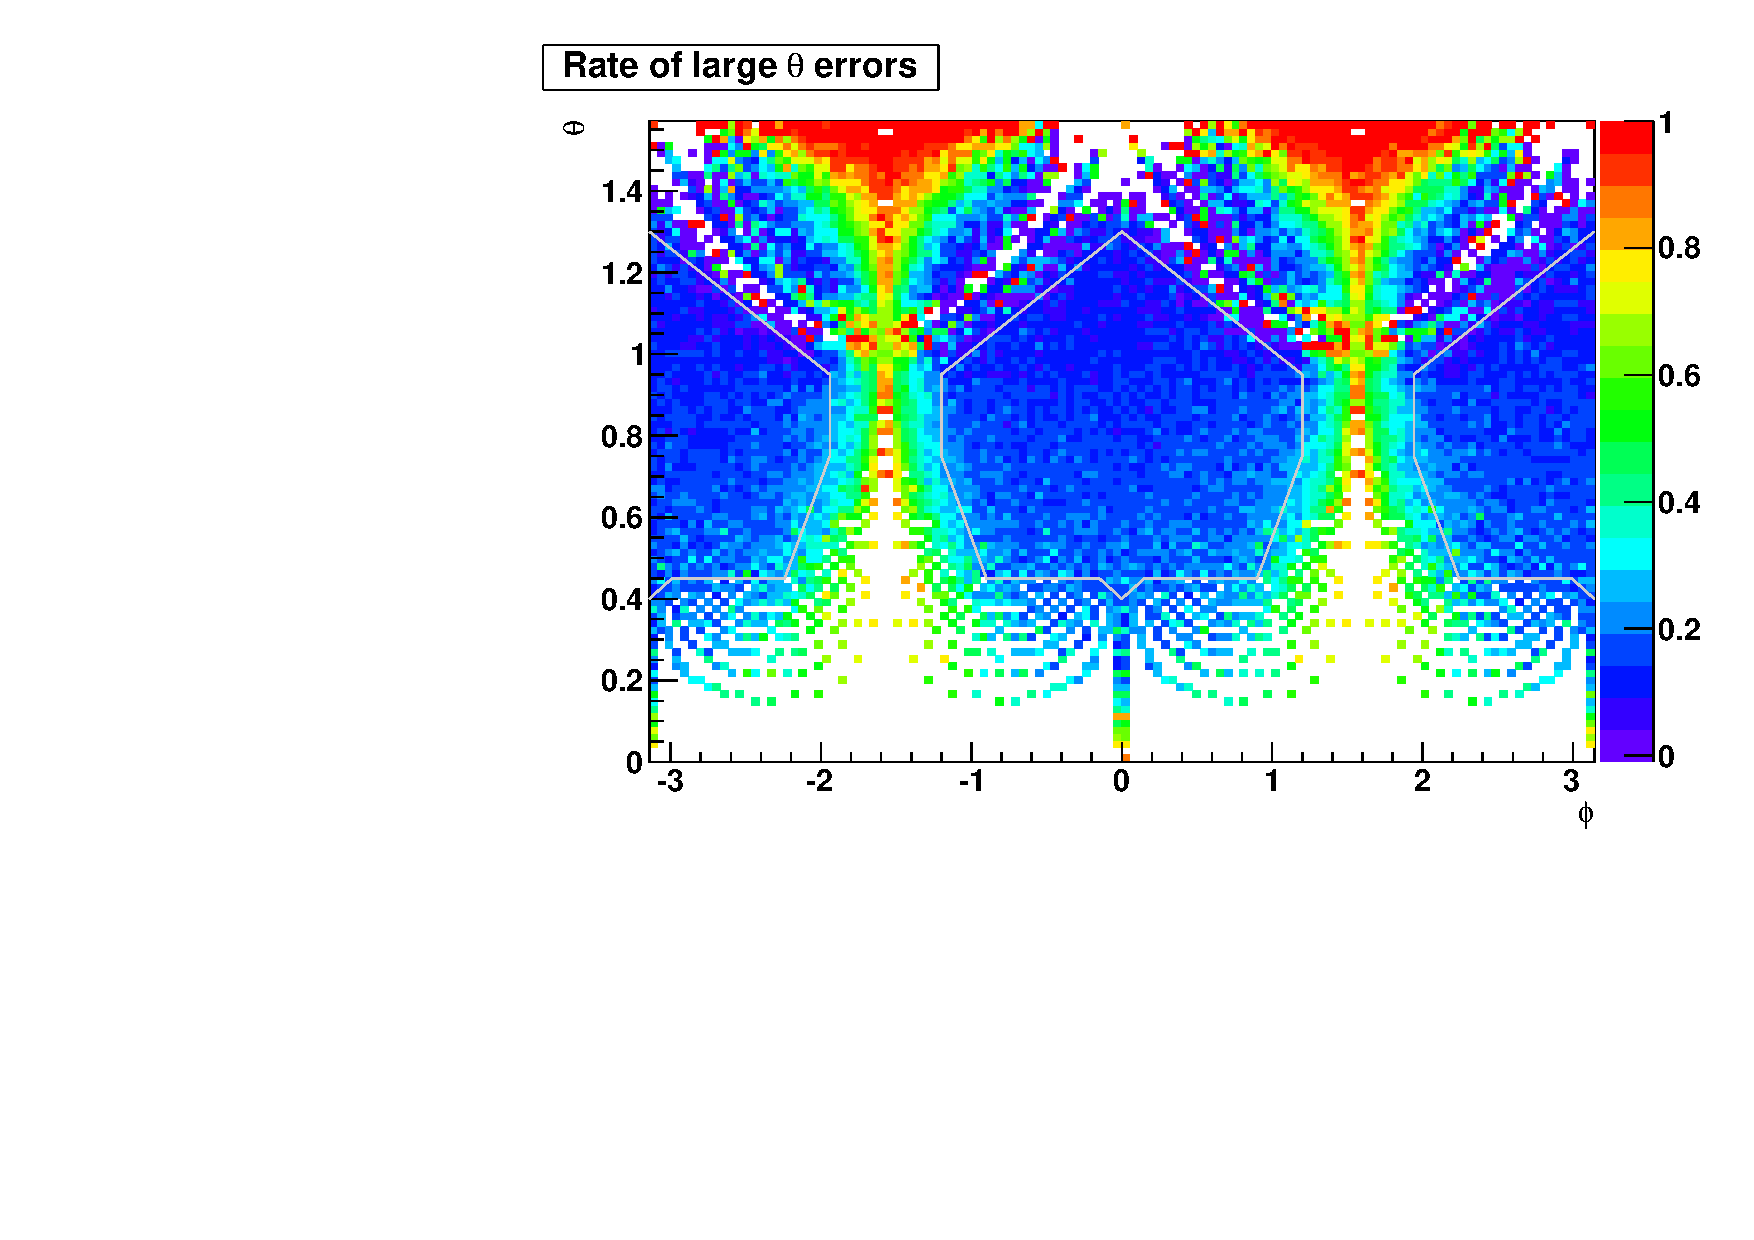
\includegraphics[width=0.8\textwidth]{./plots/muon_misrecon_theta_rate.pdf}
  \end{subfigure}
 \caption[Rate of poorly reconstructed muons]{The rate for muons to be reconstructed more than \ang{5} from their true direction. The top figure shows the rate for  errors greater than \ang{5} in total angular separation. The bottom figure shows the rate for errors greater than \ang{5} in \(\theta\) only, which is of concern because the flux varies in \(\theta\), but is isotropic in \(\phi\). The gray polygon indicates the region with good reconstruction used for this analysis. The azimuthal angle is on the horizontal axis, with \ang{3} bins, while the zenith angle is on the vertical axis, with \ang{1} bins. Blank bins had no muons reconstructed in that bin. Notice that for small \(\theta\), only a few bins are populated, indicating that angular resolution is poor for near vertical muons.}
 \label{fig:muon_misrecon_rate}
 \end{figure}

\subsection{Efficiency}
Overall, of two million simulated events, 864138 were tagged as muons by the algorithm described above. This is an overall efficiency of \(42.3 \pm 0.1\)\%. However, the geometry of the detector means that the efficiency will be a function of the incident muon angle. \Cref{fig:muon_efficiency} shows the efficiency of detecting muons based on the ratio of muons reconstructed in an angular bin to muons simulated in that bin. This is useful for estimating the true flux in a bin.

 \begin{figure}[htb]
 \centering
 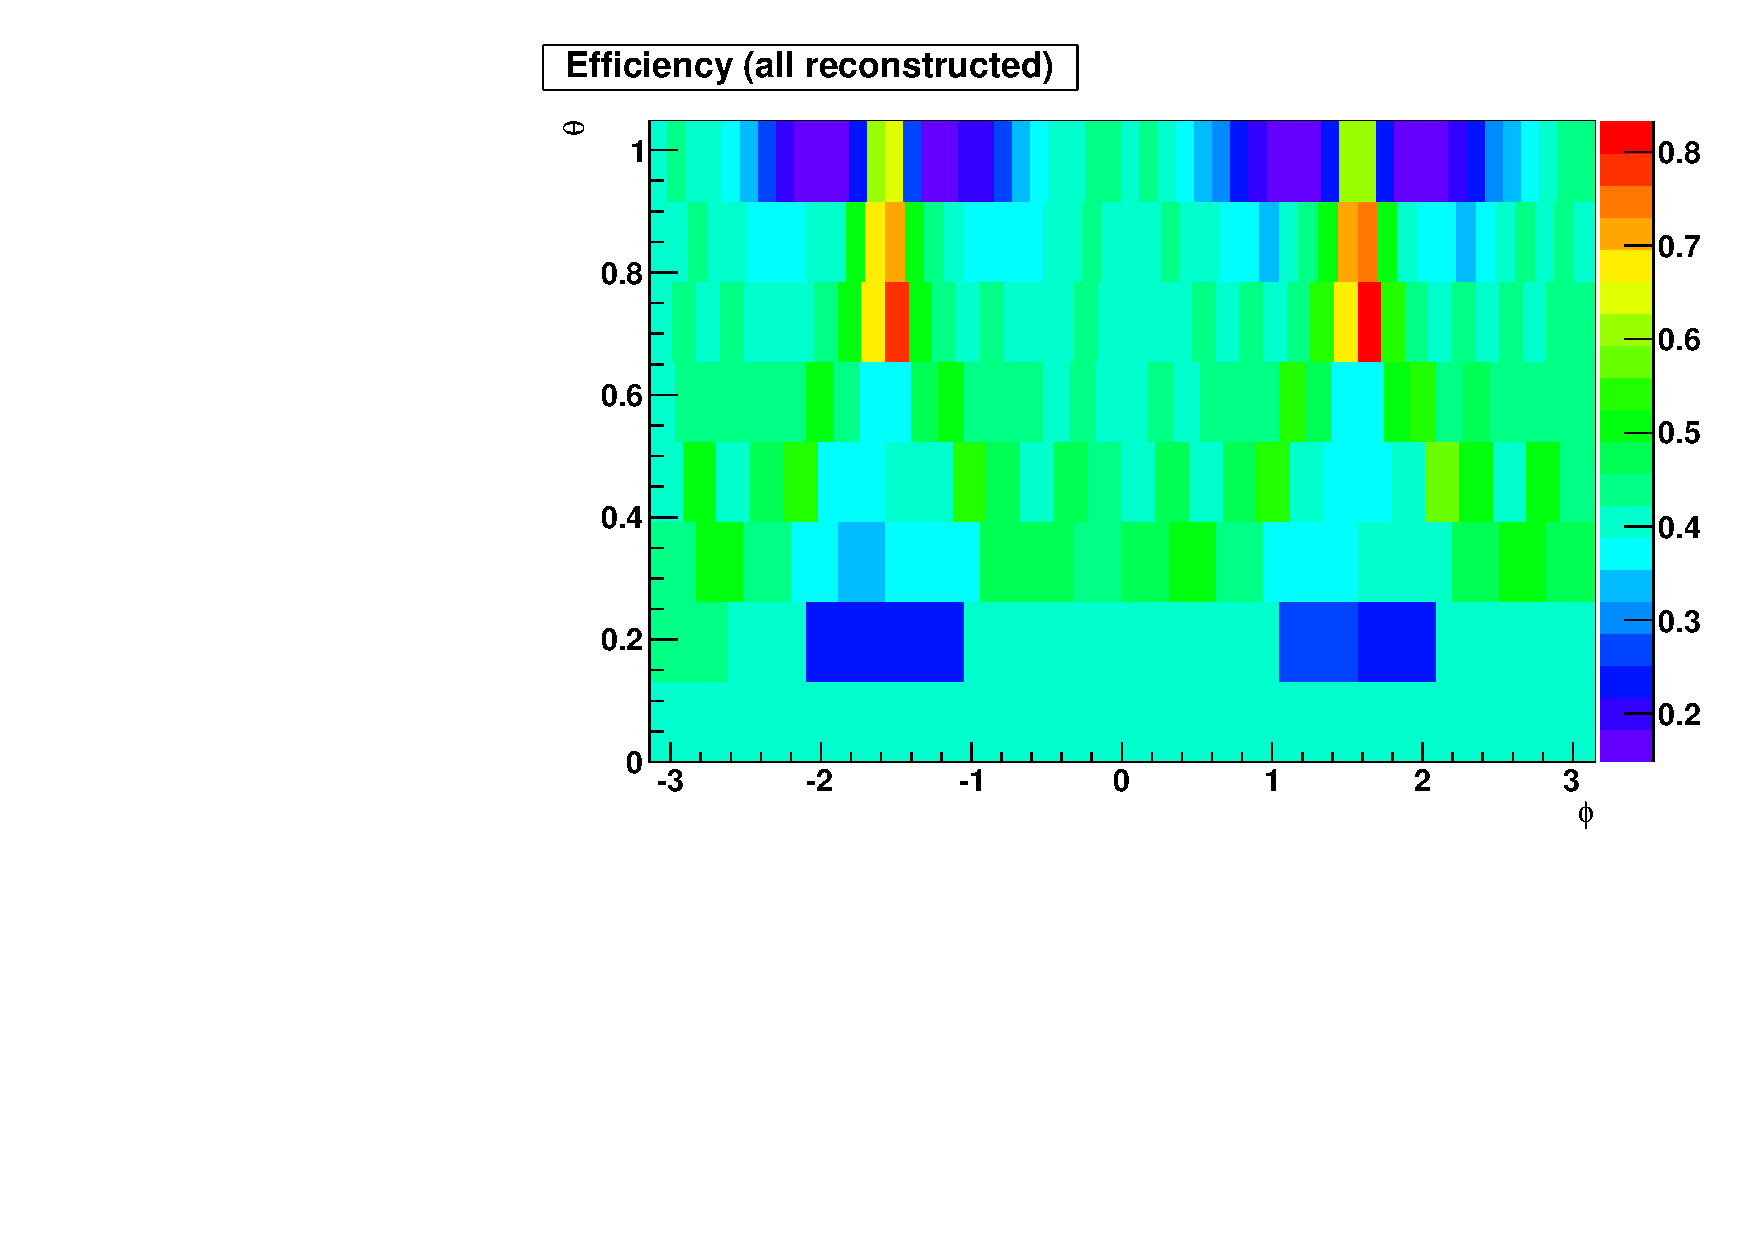
\includegraphics[width=0.8\textwidth]{./plots/muon_efficiency.pdf}
 \caption[Efficiency of reconstructing muons as a function of angle]{The ratio of muons reconstructed in an angular bin to the muons simulated in that bin. This includes muons incorrectly reconstructed, so that this can be used to estimate a total flux. The region inside the gray polygon, used for this analysis, shows reasonable efficiencies. The bin at \((\theta, \phi) = (0, 0)\) is off scale high, with a ratio of 2354, owing to poor angular reconstruction for near-vertical muons.}
 \label{fig:muon_efficiency}
 \end{figure}
 
\section{The Muon Flux at WIPP}
\label{sec:muon:wipp}
The muon flux through the  is simply
\begin{equation}
\label{eq:muon_fluxdef}
\Phi = \frac{\sum_{i}N_{\mu}}{ \Delta T\sum_{i}\Delta\Omega_i \epsilon(\theta_i, \phi_i) A(\theta_i, \phi_i)}
\end{equation}
where \(N_\mu\) is the number of muons observed in time \(\Delta T\). \(\epsilon\) is the efficiency for that bin, \(\Delta\Omega_i\) is the solid angle subtended by bin \(i\), and \(A\) is the projected area of the detector for a particle incident from \((\theta_i, \phi_i)\). The projected area of a cylinder on its side is
\begin{equation}
A(\theta,\phi) = \pi r^2 |\cos(\phi)|\sin(\theta) + 2 r \ell \sqrt{1-\sin(\theta)^2 \cos(\phi)^2}
\end{equation}
where \(r\) is the cylinder's radius and \(\ell\) is its height.

Integrating \cref{eq:muon_angular_distribution} over the polygonal region of interest, the ratio of the flux in this region to the total flux is \num{0.316\pm0.001}, where the error is found by varying the depth \(h\) by 5\% around \(1585\) \si{\hecto\gram\per\square\centi\meter}.

The pions and kaons in the atmosphere traveling with large \(\theta\) are less likely to interact as they spend more time in the low-density upper atmosphere than to decay to muons. This provides a \(\sec\theta\) enhancement in the flux underground. Therefore, most cosmic ray measurements quote a vertical muon flux:
\begin{equation}
\label{eq:muon_vfluxdef}
\Phi_v(\theta, \phi) = \Phi(\theta, \phi)\cos\theta
\end{equation}

Again integrating \cref{eq:muon_angular_distribution}, the ratio of the total flux in the region of interest to the vertical flux is \num{0.387\pm0.003}.

In data taken with the EXO-200 detector, \(12520\pm112\) muons were observed in \SI{2.140d7}{\second}. The integrated product of area, efficiency, and solid angle in the region of interest was \SI{3.359\pm0.001d3}{\per\square\centi\meter\per\steradian}. This gives a total flux of\todo{Update these numbers with new MC}
\begin{equation}
\label{eq:muon_flux_result}
\Phi = 5.76\pm0.05\text{(stat)}\pm0.01\text{(sys)}\frac{\text{Hz}}{\text{cm}^2\text{sr}}
\end{equation}
and a vertical flux of
\begin{equation}
\label{eq:muon_vflux_result}
\Phi_v = 4.24\pm0.04\text{(stat)}\pm0.01\text{(sys)}\frac{\text{Hz}}{\text{cm}^2\text{sr}}
\end{equation}

\subsection{Comparison with Previous Results}
Esch et al.\cite{Esch:2004zj} report a vertical muon flux of \((3.10^{+0.05}_{-0.07}\times10^{-7}\)\si{\Hz\per\square\centi\meter\per\steradian}. To do so, they measure a total flux and then convert it to a vertical flux using the integral of \cref{eq:muon_angular_distribution}. They calculate the ratio to be \(\Phi_v = (0.65\pm0.04)\Phi\). However, computing the integral 
\begin{equation}
\label{eq:muon_esch_integral}
\frac{\Phi_v}{\Phi} = \frac{2 \pi \int_0^{\pi/2} \varphi(h,\theta)\sin\theta\cos\theta d\theta}{2 \pi \int_0^{\pi/2} \varphi(h,\theta)\sin\theta d\theta} = 0.814^{+0.06}_{-0.05}
\end{equation}
where \(\varphi(h,\theta)\) is the distribution in \cref{eq:muon_angular_distribution} and \(h = 1526\)\si{\hecto\gram\per\square\centi\meter} (with the error due to varying this \(\pm10\%\)). The \(\sin\theta\) and \(2 \pi\) factors come from the integral over solid angle. Furthermore, the paper quotes two different values for their efficiency: \((88.5\pm0.2)\%\) and \((84.25\pm0.2)\%\). A simple toy Monte Carlo simulation with two parallel panels \SI{76.2}{\cm}\(\times\)\SI{305}{\cm} separated by \SI{30.5}{cm} with muons generated according to \cref{eq:muon_angular_distribution} yields a geometric efficiency of \((78.0^{+0.5}_{-0.4})\%\) (with the error from varying the depth \(\pm10\%\)). Correcting with this new efficiency and the correct ratio from \cref{eq:muon_esch_integral} raises the vertical muon flux observed by Esch et al. to \((4.19-4.40)\)\si{\Hz\per\square\centi\meter\per\steradian}, which agrees with the result above in \cref{eq:muon_vflux_result}.\todo{Fix this. Use their numbers, not just scale.}

%\bibliographystyle{plain}
%\bibliography{herrin-thesis}
\end{document} 